As previously explained, cvc5 has a module for exporting its proofs as Lean scripts.
We will illustrate the format used by those scripts with an instance of the SMT problem corresponding
to the negation of modus ponens, i.e. $\neg (p \rightarrow ((p \rightarrow q) \rightarrow q))$.
We present this instance using SMT-Lib~\cite{smtlib}, a standardized syntax for
representing SMT problems recognized by most SMT solvers:

\begin{minted}{smtlib2.py -x}
  (set-logic QF_UF)
  (declare-const p Bool)
  (declare-const q Bool)
  (assert (not (=> p (=> (=> p q) q))))
\end{minted}

Feeding cvc5 with this script yields the result ``unsat'', as expected. The proof produced by the solver is shown in Figure~\ref{fig:cvc5-proof} and is an instance of the resolution tree introduced in Section~\ref{sec:pcBool}.
Each node is a formula that is either from the input or was derived by applying a
rule to other nodes. An edge from some node $u$ to other node $v$ indicates that
$u$ was used to derive $v$.
In addition to the resolution rule (in purple and green), there are also rules for conjunctive normal form transformations (yellow)\footnote{The rules in the figure are in the internal calculus of cvc5, which is documented in \url{https://cvc5.github.io/docs/latest/proofs/proof_rules.html}}. Note that all leaves (in blue) correspond to the input formula, \texttt{(not (=> p (=> (=> p q) q)))}.

\makeatletter
\setlength{\@fptop}{0pt}
\makeatother

\begin{figure}[t!]
  \centering
  \scalebox{0.45}{%
    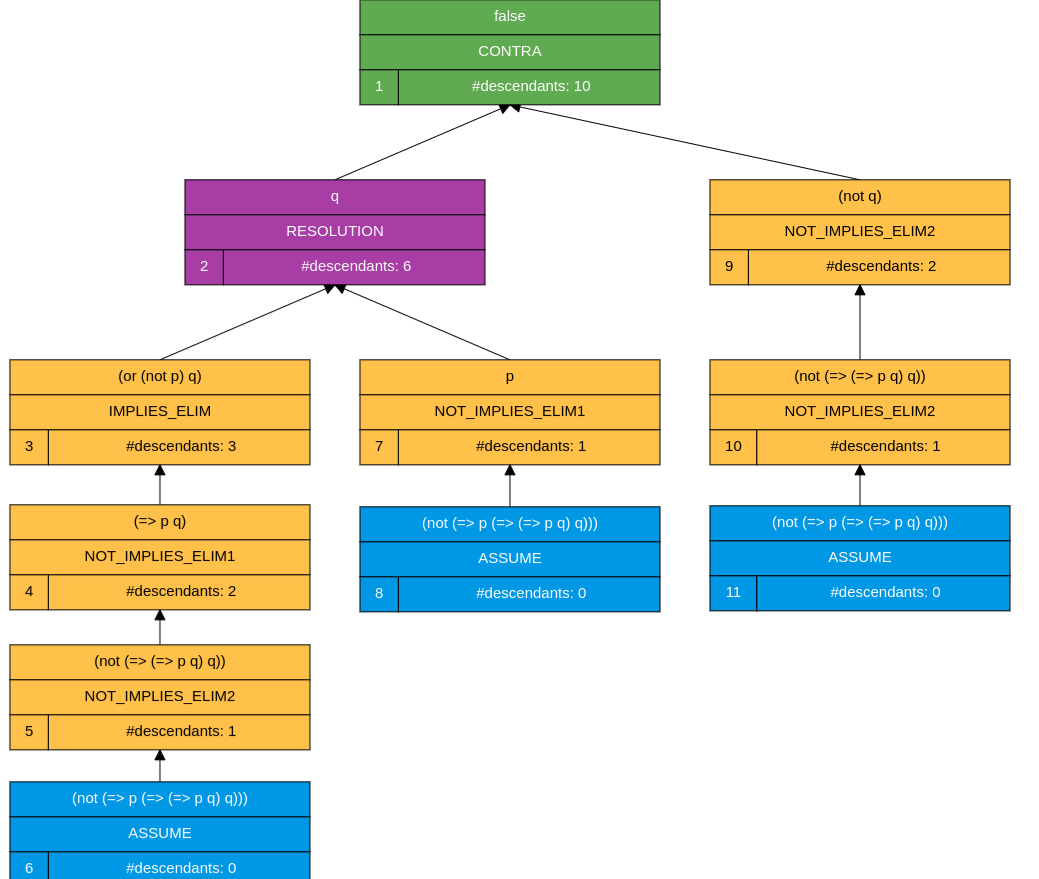
\includegraphics[scale=0.9]{img/mp_cvc5_proof.png}}
  \caption{A cvc5 proof for the validity of Modus Ponens.}
  \label{fig:cvc5-proof}
\end{figure}

The encoding of this proof into Lean requires representing the terms that appear
in it, i.e.\ the formulas built with $p$ and $q$, as well as the rules.
%
This encoding uses a \emph{deep embedding} of the proof calculus of cvc5 into
Lean\footnote{The code is available at \url{https://github.com/tomaz1502/signatures/blob/smallCheckers/Cdclt/Lift/Other/PropsExample.lean}}.
%
It provides a \texttt{term} type that models terms and formulas from MSFOL. This type has
a \texttt{const} constructor for defining symbols, parameterized with an
identifier (a natural number) and a \texttt{sort} (another type for encoding MSFOL
sorts).
%
For example, \texttt{p} and \texttt{q}, which are Boolean constants (MSFOL
constants can be seen as free variables when they are not pre-defined, which is
the case for \texttt{p} and \texttt{q} but not for example for \texttt{false}),
are declared as:

\begin{minted}{lean}
  def p: term := const 1000 boolSort
  def q: term := const 1001 boolSort
\end{minted}

The identifiers \texttt{1000} and \texttt{1001} are arbitrary, with only the
requirement that they are unique.

With these terms and using the functions \texttt{implies} and
\texttt{not} defined in the deep embedding corresponding to the MSFOL symbols
$\rightarrow$ and $\neg$, we encode the formula used in the
query:

\begin{minted}{lean}
  def modusPonensEmbed: term := implies p (implies (implies p q) q)
  def notModusPonensEmbed: term := not modusPonensEmbed
\end{minted}

Finally, the proof from Figure~\ref{fig:cvc5-proof} is encoded as:

\begin{minted}{lean}
  theorem cvc5_th0 : thHolds notModusPonensEmbed -> thHolds bot :=
    fun lean_a0 =>
      have lean_s0 := notImplies2 lean_a0
      have lean_s1 := notImplies1 lean_s0
      have lean_s2 := impliesElim lean_s1
      have lean_s4 := notImplies1 lean_a0
      have lean_s6 := R1 (conjunction lean_s2 lean_s4)
      have lean_s9 := notImplies2 lean_s0
      contradiction (conjunction lean_s9 lean_s6)
\end{minted}
where \texttt{thHolds} is a Lean axiom that lifts a \texttt{term} into a \texttt{Prop}, asserting that it is a valid term.
All the inference rules are encoded as axioms that have the type \texttt{thHolds t1 -> thHolds t2}, for some terms \texttt{t1} and \texttt{t2}. For instance, \texttt{notImplies1} is written in the following form:
\begin{minted}{lean}
  axiom notImplies1 : ∀ {t1 t2 : term},
    thHolds (not (implies t1 t2)) -> thHolds t1
\end{minted}
where the usage of curly brackets indicate that the parameters are implicit.

By applying the rules in the sequence generated by cvc5, we can derive a term
that has type \texttt{thHolds notModusPonens -> thHolds bot}, where \texttt{bot}
is the encoding of MSFOL's \texttt{false}.
%
The existence of this term shows that, assuming the rules used by cvc5 are correct, the term \texttt{notModusPonens} is equivalent to \texttt{bot}, which is the same as to say that it is unsatisfiable. This way, we have encoded the proof found by cvc5 inside Lean.

Note that the encoding and printing of the SMT-Lib query as a \texttt{term}, as well as the encoding and printing of the proof, are done automatically by cvc5. On the other hand, the definition of the type \texttt{term} and the declaration of the axioms corresponding to the rules remain static within the module.
